\documentclass[12pt, a4paper, oneside]{ctexbook}
\usepackage{amsmath, amsthm, amssymb, bm, graphicx, hyperref, mathrsfs, enumitem, geometry, listings, fontspec, ,xcolor}

\title{{\Huge{\textbf{《电子商务应用》}}}\\实验报告}
\author{徐鸣飞、黄梓霖、皮佳宇、陈其阳}
\date{\today}
\linespread{1.5}
\newtheorem{theorem}{定理}[section]
\newtheorem{definition}[theorem]{定义}
\newtheorem{lemma}[theorem]{引理}
\newtheorem{corollary}[theorem]{推论}
\newtheorem{example}[theorem]{例}
\newtheorem{proposition}[theorem]{命题}

\lstset{ %
    numbers=left, %设置行号位置
    numberstyle=\tiny, %设置行号大小D:\LaTeX\workspace\homework\软件需求\main.pdf
    keywordstyle=\color{blue}, %设置关键字颜色
    commentstyle=\color[cmyk]{1,0,1,0}, %设置注释颜色
    frame=single, %设置边框格式
    escapeinside=` `, %逃逸字符(1左面的键),用于显示中文
    breaklines=true, %自动折行
    extendedchars=false, %解决代码跨页时,章节标题,页眉等汉字不显示的问题
    xleftmargin=2em,xrightmargin=2em, aboveskip=1em, %设置边距
    tabsize=4, %设置tab空格数
    showspaces=false %不显示空格
}

\geometry{a4paper,scale=0.7}
\begin{document}

\maketitle

\pagenumbering{roman}
\setcounter{page}{1}

% \begin{center}
%     \Huge\textbf{前言}
% \end{center}~\

% 这是笔记的前言部分. 
% ~\\
% \begin{flushright}
%     \begin{tabular}{c}
%         Dylaaan\\
%         \today
%     \end{tabular}
% \end{flushright}

\newpage
\pagenumbering{Roman}
\setcounter{page}{1}
\tableofcontents
\newpage
\setcounter{page}{1}
\pagenumbering{arabic}

\chapter{概述}
\section{关键字广告与竞争性营销}
关键词广告(keyword)是一种文字链接型网络广告,通过对文字进行超级链接,让感兴趣的网民点击进入公司网站、网页或公司其它相关网页,实现广告目的。链接的关键词既可以是关键词,也可以是语句。

竞争性营销:在营销管理过程中,管理者不仅要考虑顾客的需要,还要考虑企业在本行业中的竞争地位。企业的营销战略和战术必须从自己的竞争实力地位出发,并根据自己同竞争者实力对比的变化,随时加以调整,使之与自己的竞争地位相匹配。由于现代市场营销中竞争的重要性,市场营销不仅包括“产品、价格、促销、渠道”四方面因素,还应让“竞争”成为现代市场营销的第五大因素。竞争意识要在企业的营销决策、营销规划、营销组织中充分体现出来,在营销实践中也要采取有效的策略开展竞争,不断提高企业竞争能力。
\section{关键字推荐方法}
设所有关键词全集为:$K$,

广告主的种子关键词:$ s \left( s \in K \right) $,

推荐高相关性的关键词:$ K_M \left( K_M \in K \right) $。

\begin{itemize}
    \item 相关分析法:计算词与词之间的相关程度:

    \begin{enumerate}
        \item 关联相关性:指的是两个关键词之间的相关性,通常是指它们在同一文本中出现的频率或者它们之间的语义关系。例如,在一篇文章中,如果两个关键词经常同时出现,那么它们之间就有很强的关联相关性。
        \item 同义词相关性:指的是两个关键词之间的同义词关系。例如,“汽车”和“车辆”就是两个同义词,它们之间有很强的同义词相关性。同义词相关性通常需要通过词汇库或者自然语言处理技术来识别。
        \item 竞争相关性:指的是两个关键词之间的竞争关系。例如,在搜索引擎中,如果用户搜索“手机”,那么“苹果”和“三星”就是两个与“手机”相关的竞争关键词。竞争相关性通常需要通过分析用户搜索行为或者竞争对手的关键词来识别。
    \end{enumerate}

    \item 方法:
    \begin{figure}[htbp]
        \centering
        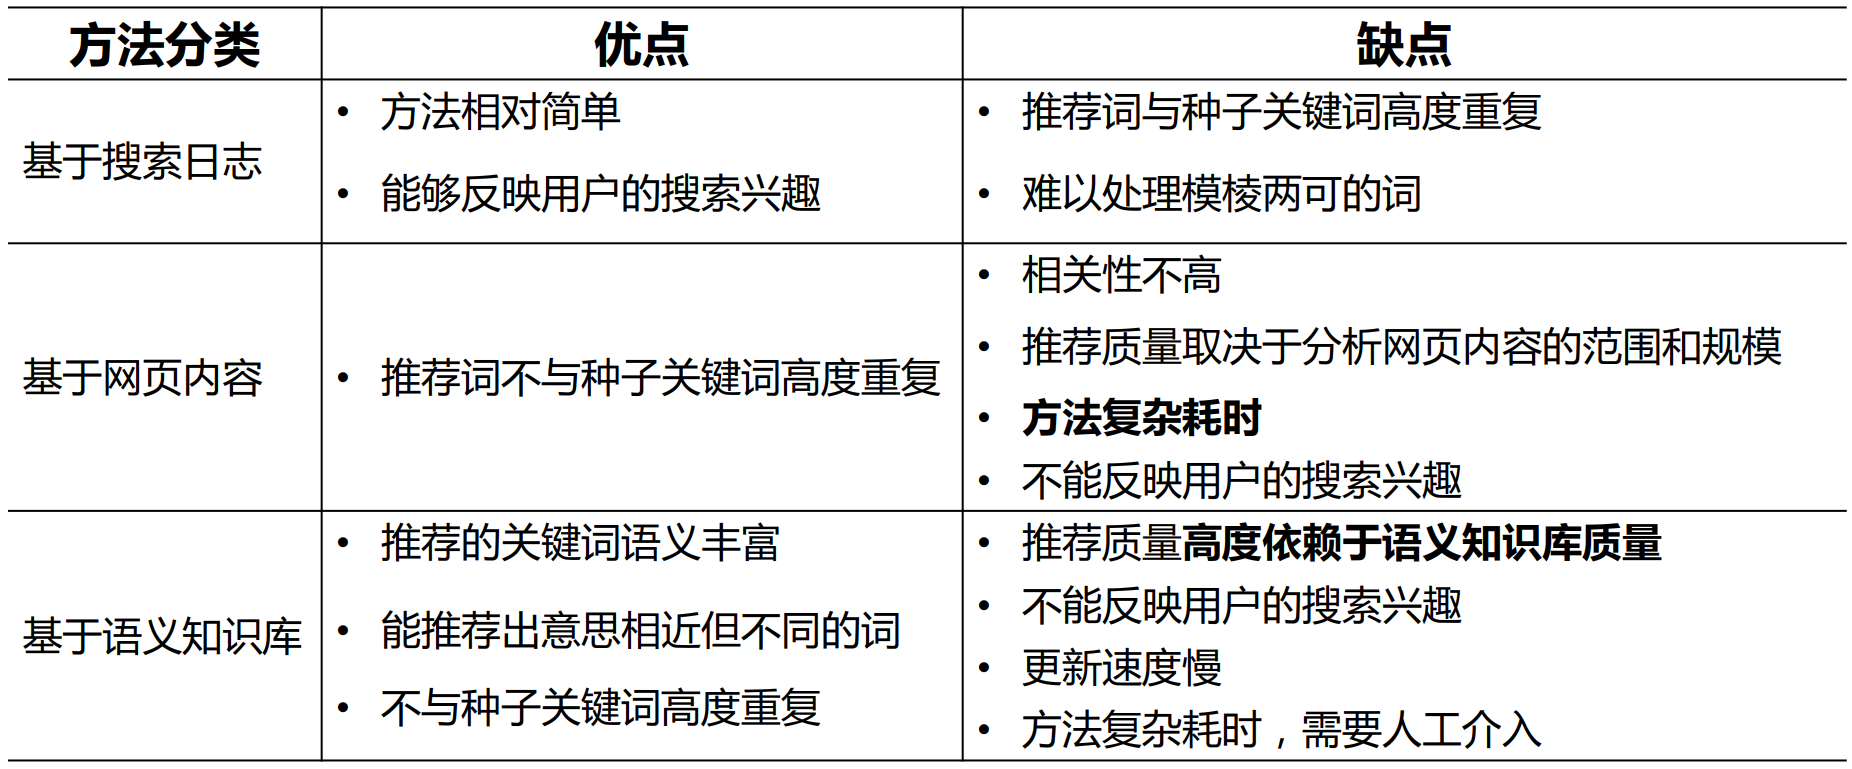
\includegraphics[height = 6cm, width = 15cm]{方法.png}
        \caption{关键词推荐方法比较}
        \label{fig:example}
    \end{figure}

    \item 通过了解用户搜索意图来获得$ K_M $
\end{itemize}

\section{竞争性关键字与度量方法}
构建相应的概率模型来计算关键字之间的竞争度:
\vspace{20pt}

    \begin{minipage}{0.4\textwidth}
        \begin{equation*}
            Comp_a\left(k,s\right)=\frac{|{ka}|}{(|{a}|-|{sa}|)}
        \end{equation*}
    \end{minipage}
    \hfill
    \begin{minipage}{0.5\textwidth}
        \begin{itemize}[itemsep=0pt,parsep=0pt,partopsep=0pt,topsep=0pt]
        
            \item s:种子关键字
            \item k:任意关键词
            \item a:中介关键词
        \end{itemize}
    \end{minipage}
    
\vspace{20pt}
\begin{itemize}
    \item 种子关键词 $s$ 与任意关键词 $k$ ,存在一个中介关键词 $a$ ,其与 $s$ 与 $k$ 都存在联合查询,即 $sa$ 与 $ka$。
    \item 度量了在所有查询 $ka$ 的搜索量占 $a$ 搜索量中除去 $sa$ 搜索量的比例,反映了在 $a$ 关键词的维度上,用户不搜索 $k$ 而搜索 $s$ 的概率。
\end{itemize}

多个中介关键词存在程度的竞争性, $a$ 对于 $k$ 的影响权重:
$$W_a(k)=\frac{|{sa}|}{|{s}|}$$

关键词与种子关键词的竞争性程度:
$$Comp(k,s)=\sum_{i=1}^{m}\left\{w_{ai}(k)\times Comp_{ai(k,s)}\right\}$$

\section{设计与实现的技术线路}
\begin{enumerate}
    \item 操作系统:Windows 10 家庭中文版。
    \item 软件环境:JDK 1.8 + word 1.3
    \item 设计与实现:
    \begin{itemize}
        \item \textbf{总体流程}:清洗数据,获取所有关键词;compkey算法开始,输入种子关键词,如:“湖南”;接着从总搜索量中提取出与种子关键词相关的所有搜索信息;对与种子关键词相关的搜索信息进行分词与词频统计;通过对词频统计信息分析确定一定数目的中介关键词;对每个中介关键词查找相应的竞争性关键词,并计算竞争度;最后统计输出,结果保存到文件中。
        \item \textbf{中介关键词的选取}:对于一个确定的种子关键词,对清洗后的数据进行提取,得到与种子关键词有关的所有的搜索量保存到文件中,使用word分词插件对该文件进行分词与词频统计,出现的次数越多说明相关性越大,权重越大,则可以选取出现频率高的词作为中介关键词。
        \item \textbf{竞争关键词的选取}:每一个中介关键词都会对应一个竞争性关键词。对于每一个确定的中介关键词,从清洗后的数据中进行提取出于中介关键词有关的所有的搜索量保存到文件中,使用word分词插件对该文件进行分词与词频统计,出现的次数越多说明其与中介关键词相关性越大,则可以选取出现频率最高的词(该词不是种子关键词和中介关键词)作为竞争关键词。
    \end{itemize}
\end{enumerate}

\chapter{关键词竞争算法数据预处理}
\section{数据来源与数据特征}
\begin{enumerate}
    \item 数据来源:C:\textbackslash Users\textbackslash 24964\textbackslash Desktop\textbackslash mavenproject1 \textbackslash data\textbackslash 搜狗比赛数据
    
    \textbackslash user\_tag\_query.10W.TRAIN
    \item 数据特征(字段说明):数据特征(字段说明)
    \begin{itemize}
        \item \textbf{ID}:加密后的ID
        \item \textbf{age}:0:未知年龄; 1:0-18岁; 2:19-23岁; 3:24-30岁; 4:31-40岁; 5:41-50岁; 6:51-999岁
        \item \textbf{Gender}:0:未知 1:男性 2:女性
        \item \textbf{Education}:0:未知学历; 1:博士; 2:硕士; 3:大学生; 4:高中; 5:初中; 6:小学
    \end{itemize}
    \item 数据示例:00627779E16E7C09B975B2CE13C088CB\ 4\ 2\ 0钢琴曲欣赏100首\ 一个月的宝宝眼睫毛那么是黄色\ 宝宝右眼有眼屎\ 小儿抽搐怎么办\ 剖腹产后刀口上有线头\ 属羊和属鸡的配吗
\end{enumerate}
\section{种子关键词的选取}
"作文", "小说", "大学", "软件", "工资", "诗句", "电视剧", "广场舞", "手机", "壁纸"
\section{数据获取与关键代码实现}
\begin{lstlisting}
public class MainDataClass {
    public static void data(String wordKey) throws FileNotFoundException, UnsupportedEncodingException, IOException, Exception {
        PathClass pa = new PathClass();
        InputStreamReader inStream = new InputStreamReader(new FileInputStream(new File(pa.wordOut)), "utf-8");//读取总搜索量文件
        OutputStreamWriter outStream = new OutputStreamWriter(new FileOutputStream(new File(pa.wordRelated)), "utf-8");
        BufferedReader bf = new BufferedReader(inStream);
        BufferedWriter bw = new BufferedWriter(outStream);
        String valueString = null;
        while ((valueString=bf.readLine())!=null){  //与种子关键字相关的搜索信息
            if(valueString.contains(wordKey)) {
                bw.append(valueString);
                bw.newLine();
            } 
        }
        bw.close();
        File f = new File(pa.wordRelated);
        if(f.length() == 0) {
            System.out.println("搜索日志中不含关键词“" + wordKey +"”,请重新设置种子关键词!!!");
            System.exit(0);
        }
        System.out.println("加载Word分词器...");
        System.out.println("开始对与种子关键字相关的搜索信息进行分词与词频统计...");
        new StatisticsDataClass().statistic(pa.wordRelated, pa.wordApart, pa.wordStatistics);//对相关信息进行分词和词频统计
    }
}
public class StatisticsDataClass {
    public static void statistic(String wordOut, String wordApart, String wordStatistics) throws Exception {
        //词频统计设置
        PathClass pa = new PathClass();
        PrintStream ps = new PrintStream(pa.log);/*过滤屏幕信息*/
        PrintStream out = System.out;
        System.setOut(ps);
        WordFrequencyStatistics wordFrequencyStatistics = new WordFrequencyStatistics();
        wordFrequencyStatistics.setRemoveStopWord(true);//去掉虚词和一般的连词
        wordFrequencyStatistics.setResultPath(wordStatistics);
        wordFrequencyStatistics.setSegmentationAlgorithm(SegmentationAlgorithm.MaxNgramScore);
        wordFrequencyStatistics.seg(new File(wordOut), new File(wordApart));
        wordFrequencyStatistics.dump();//输出词频统计结果
        System.setOut(out);
        wordFrequencyStatistics.dump();
    }
}
\end{lstlisting}
\section{预处理后的数据格式}
换行后结果:见图\ref{fig:example1}
分词后结果:见图\ref{fig:example2}
统计词频率结果:见图\ref{fig:example3}
\begin{figure}[htbp]
    \centering
    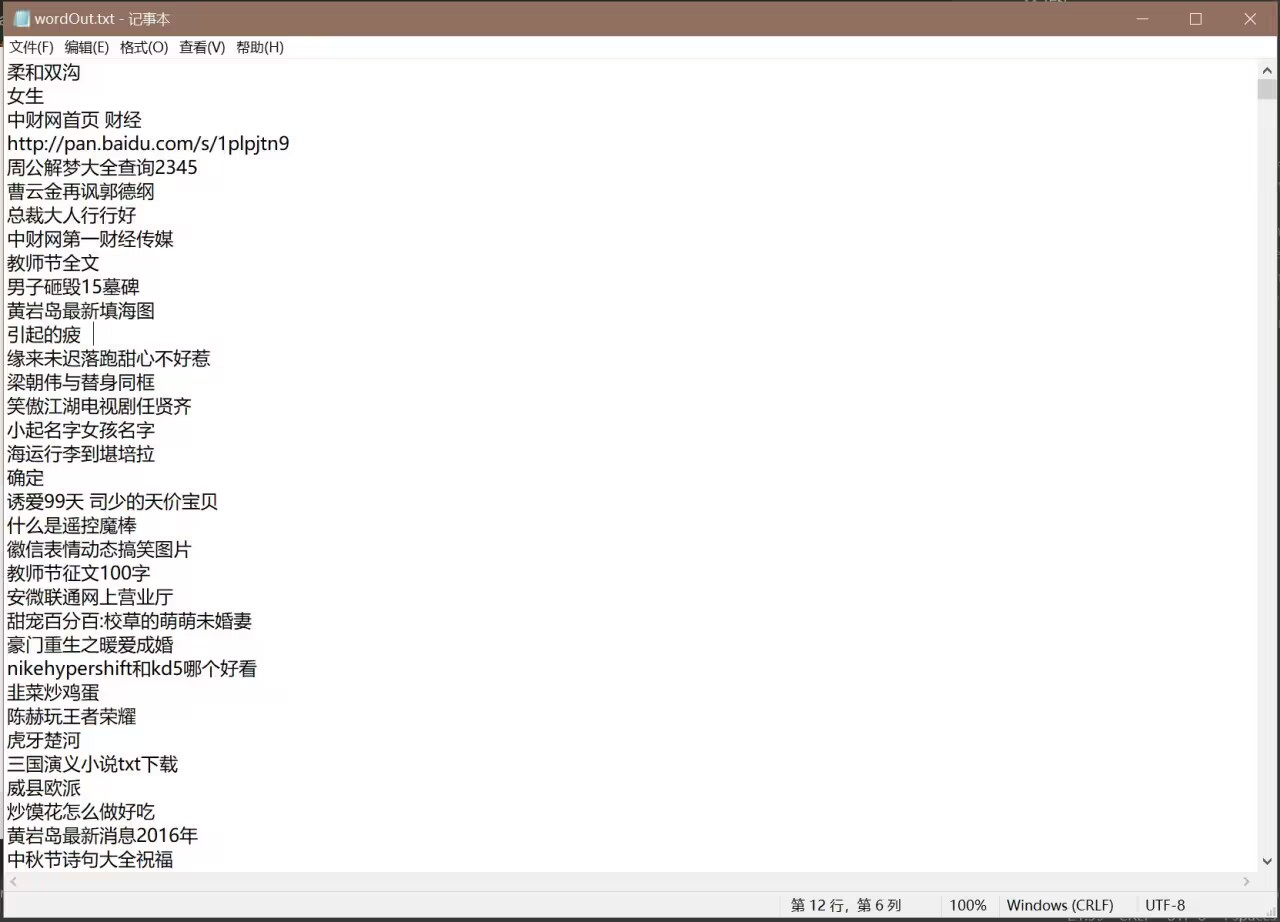
\includegraphics[scale=0.3]{换行.jpg}
    \caption{换行结果}
    \label{fig:example1}
\end{figure}
\begin{figure}[htbp]
    \centering
    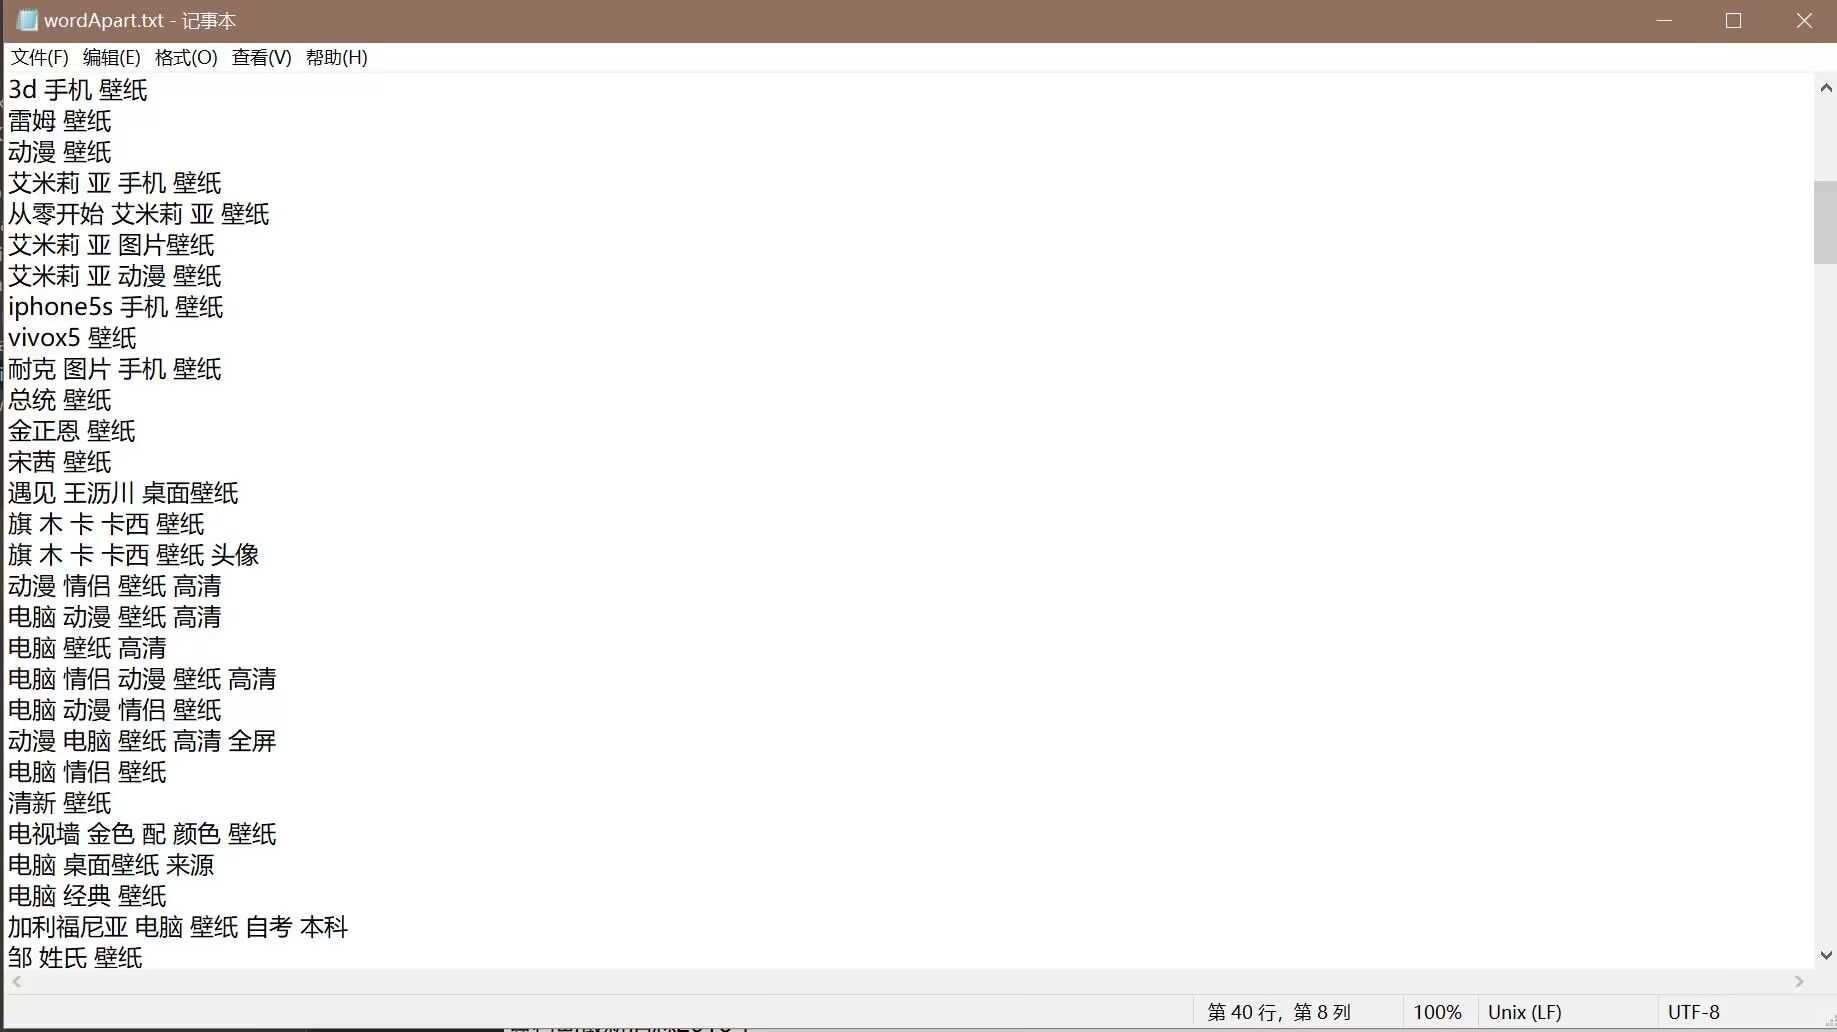
\includegraphics[scale=0.2]{分词.jpg}
    \caption{分词结果}
    \label{fig:example2}
\end{figure}
\begin{figure}[htbp]
    \centering
    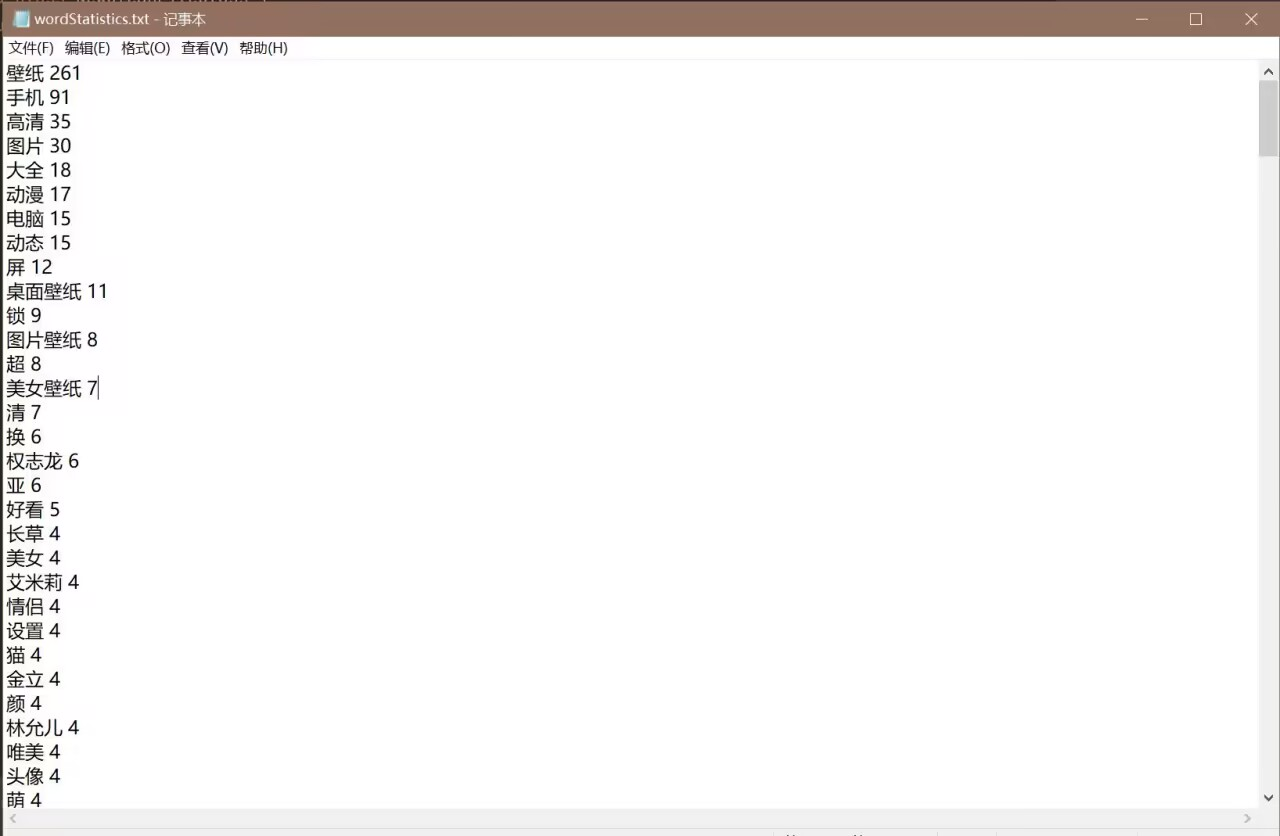
\includegraphics[scale=0.3]{词频.jpg}
    \caption{词频统计结果}
    \label{fig:example3}
\end{figure}
\end{document}
